\documentclass[pageno]{jpaper}

%replace XXX with the submission number you are given from the ASPLOS submission site.
\newcommand{\asplossubmissionnumber}{684}

\usepackage[normalem]{ulem}

\begin{document}

\title{A Study of Energy Efficiency in Operating Systems \\ \textbf{Extended Abstract}}

\date{}

\maketitle

\thispagestyle{empty}

% No abstract needed for the extended abstract
%\begin{abstract}
%\end{abstract}
%
%
%
\section{Motivation: Energy Efficiency}

Monitoring and reducing the energy consumption of servers in data centers is critical.
Reducing the power drawn by 10,000 datacenter servers by 10 watts (10 joules/second) would result in significant energy savings that could power approximately 100 US households with a corresponding financial saving of \$100,000/year\footnote{\textbf{(provide details of calculation)}}.

A server's energy use is related to the complex interactions between the application workload,  software stack, and the hardware characteristics and configuration of the server node itself.
In this work, we shed light on
the task of tuning hardware parameters to control the time and energy required for IO sensitive, system-centric workloads typical of cloud services.
We reveal the significant impact that static  tuning can have and the influence of operating systems software on the energy efficiency, specifically that of cloud-like network applications.

\section{State of the Art on Energy Efficiency}

General purpose operating systems (OSes), such as Linux, have been designed and implemented to support a broad range of user software as well as the concurrent execution of competing applications. Thus, they have evolved to include support for dynamically adjusting various hardware settings.
Dedicating a node provided by a cloud service to a single application suggests that one may be able to manually tune the node's hardware parameters to fixed values and obtain higher efficiency than allowing the OS to dynamically adjust them.  It is also possible that the impact of such hardware tuning can be magnified if one starts with an application specific OS (referred to as library OS ~\cite{ebbrt,ix,arrakis, exokernel} or unikernels~\cite{rumpkernel, unikernels}) that has been designed and implemented for running a single dedicated application.

Studying the energy saving potential that results from tuning hardware parameters such as Dynamic Voltage Frequency Scaling (DVFS) and Running Average Power Limit (RAPL) to specific values has been explored in the context of processor and memory bound co-located applications (~\cite{10.1145/3177754, zhang2015quantitative,10.1145/3302424.3303981}).
Particularly, recent works explore energy proportional computing under strict SLA objectives when applied to in-memory key-value stores using both general purpose and specialized library OSes ~\cite{10.1145/2678373.2665718, 10.1145/2806777.2806848, rubik, 10.1145/2806777.2806848}.
Other research emphasizes the importance of taking advantage of sleep states to save energy ~\cite{powernap,10.1145/3302424.3303981}.

\section{Goals}
\begin{figure}
  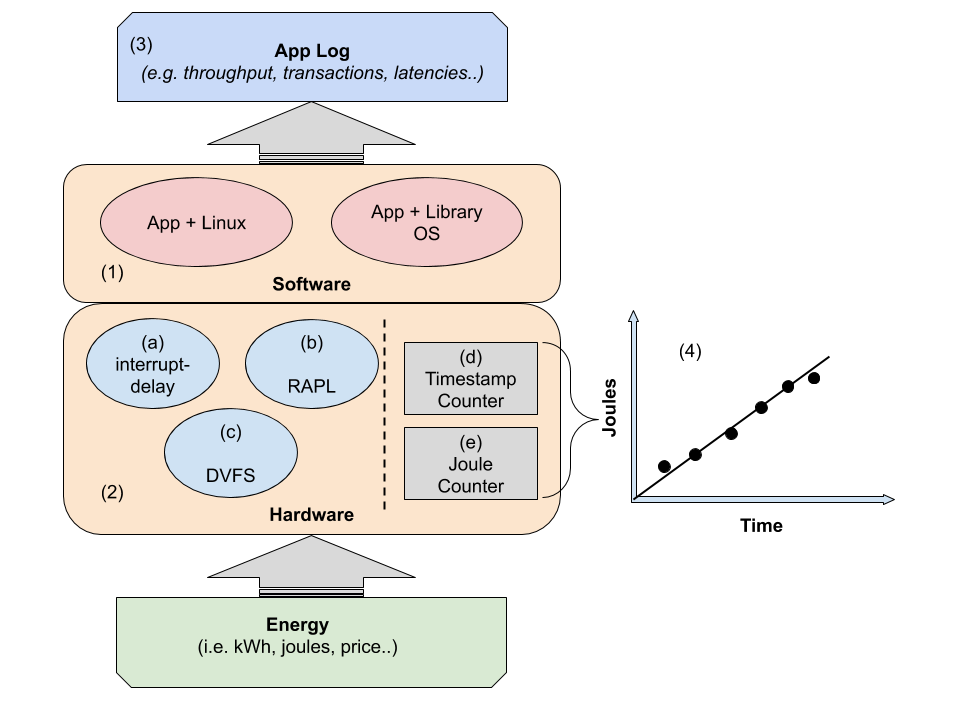
\includegraphics[width=8.5cm]{figures/setup.png}
  \caption{}
 \label{fig:setup}
\end{figure}
Our work presents fine-grained, per-interrupt energy and time analysis for network-bound, cloud-like applications. We presents the results of manually tuning three hardware parameters across four network applications and on two distinct OSes.
Figure~\ref{fig:setup} illustrates our experimental overview of this tuning task.
We do so by developing a novel methodology for understanding the impact of hardware tuning on systems and systems software.
Our results in tuning processor and NIC parameters illustrate the importance and impact of holistic system optimization of processors, memory and storage toward an energy proportional goal and the advantage of pairing that optimization with the use of specialized, baremetal library OSes.


\section{Overview of Experimental Approach}

We present the results of manually tuning three hardware parameters across four network applications and on two distinct OSes.
We begin with a study of a simple network scenario in which two systems are configured to exchange a single stream of packets of a fixed size.  We then describe our study of a NodeJS webserver driven by a single stream of sequential request over a persistent connection.  Moving up in complexity, we present results from our multicore memcached study under a stringent SLA objective. Finally, we present results from exercising a server running the Silo in-memory database combined with memcached.

We compare the results to baseline data gathered using Linux configured to its default behaviour: default values for the three hardware parameters (two of them are  dynamically adjusted using algorithms while the third is has a default fixed value).
We evaluate and compare this tuning by adapting the energy delay product (EDP) (energy used multiplied by delay) metric from the architecture community.
We use a workload-specific measure (e.g. number of message round-trips or web requests) to define work done on computational nodes and define delay as the time taken to do this work and energy as the joules consumed in the process.
Finally, we use the value of EDP on each system as an indicator of energy efficiency.

\section{Main Contributions}

The contributions of this paper are as follows:
\begin{itemize}
    \item A new methodology for the detailed study of energy consumption including the interaction of systems software.
    \item An adaption and application of EDP to the study of complex IO intensive software stacks.
    \item A quantification of the impact of jointly tuning network interrupt delay, DVFS, and RAPL on Linux's energy consumption compared to its default dynamic policies.
    \item Exposure of the dramatic benefits of statically tuning hardware parameters for dedicated workloads on Linux.
    \item A novel quantification of the benefits on energy consumption of using a baremetal application-specific library OS.
\end{itemize}


\section{Insight and Key Results}
We are the first to quantify the impact of using baremetal library OS on energy by collecting fine-grained per interrupt statistics of using both packet processing and hardware counters.  We find that the library OS uses fewer instruction to complete the work and that this has impact on the energy consumed.  This largely translates into getting more application level work done in fewer instruction.  High speed data center networks put the OS and protocol stack processing code on the hot path. Using fewer instructions (and attendant drop in busy cycles) to complete the application work leads to two energy consumption benefits; 1) it reduces the base energy cost to complete the work, and 2) it creates greater opportunities to halt the processor between network transactions.  The later benefit makes it possible to achieve a simple "race to halt" behaviour across epochs of network activity and enables going into processor sleep states. We also find that across all our applications, the simplified and naive policies of the library OS leads to taking advantage of faster sleep state transitions while also achieving higher performance. This is due in part to the library OSes packet processing efficiency to get work done quickly and therefore go into a deep sleep state.

%\footnote{Processors typically support a range of sleep states where deeper sleep states result in less energy consumption but have higher latency and potential performance penalties when waking up.} till the next interrupt.  The actual period that one can sleep for depends on the workload and the optimization criteria being imposed (eg. latency versus throughput).   

 %In the library OS, when an interrupt occur it implements a default run to completion model, by disabling interrupts.  When there are no work, pending interrupts or packets de-queued from prior interrupts to process, then the library OS simply halts the processor to the deepest available sleep state. 
\begin{figure}
	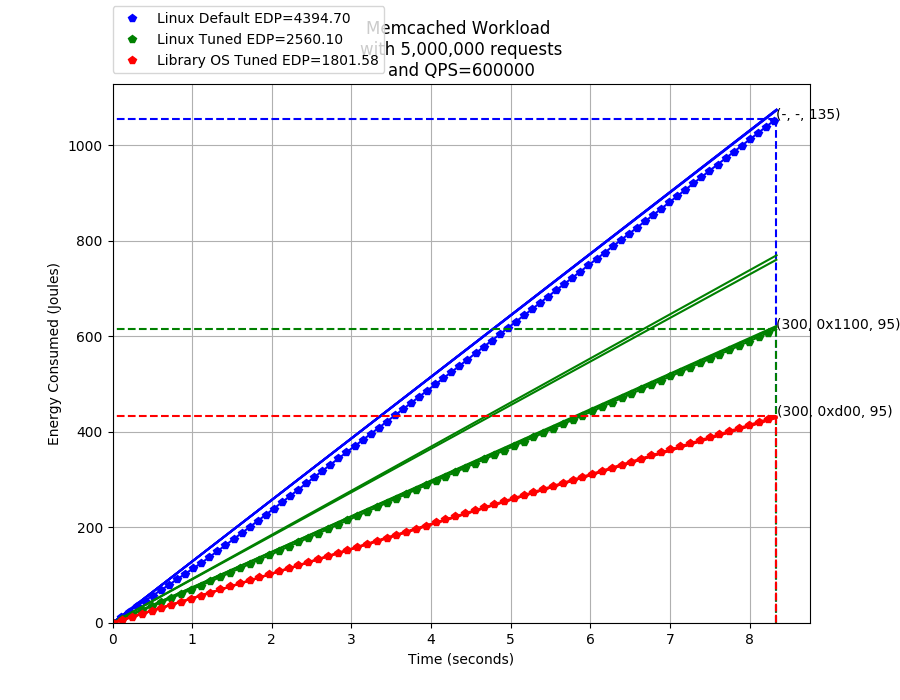
\includegraphics[width=\columnwidth]{asplos2021_figures/mcd_edp_QPS600000.png}
	\caption{Minimum EDP plots when tuned for lowest energy use in memcached at QPS 600K while maintaing 99\% SLA < 500 $\micro$s.}
	\label{fig:mcd600K}
\end{figure}

%In contrast, even though we disable Linux's mechanisms for setting the parameters, there are other complex algorithms and policies that affect its behaviour.  For example Linux application processing runs with interrupts enabled, it implements a complex algorithm for enacting a hybrid polling versus interrupt processing across network devices and has a subtle infrastructure for deciding what sleep state should be used for halting the processor based on estimation of when the next interrupt will occur from any source.  This all contributes to a complex dynamic behavior with respect to when the system should halt and if it does halt what sleep state will be requested.  We observed that even after we use fixed values for the three hardware parameters, the other complex behaviours of Linux limits its ability to tune its combined energy and performance as efficient as the library OS

%The components of cloud services such as cache servers, javascript webservers, and in-memory data bases, are  by their nature are network driven.  induce vary degrees of processor work.  Their operation and thus their efficiency is a complex mixture of the behaviour of the system software and the application software. 
%Linux's network device driver uses a dynamic algorithm that seeks to tune the interrupt delay value such that it better reflects the current workload.
%It achieves this by using data received from the previous interrupt about packet counts and bytes per packet. It is possible to disable this dynamic algorithm through the flip of a bit inside the device driver. After flipping this bit, \textit{ethtool} can then be used to set new interrupt delay values to statically fire at a fixed rate. This hardware parameter exposes another set of trade-offs for network applications.
%received from the last interrupt and classifies them broadly into a set of ranges that are pre-computed based off theoretical maximum wire speeds.
%This delay tuning is applied upon the next interrupt occurrence.


%While NICs have many adjustable parameters, interrupt-delay, the amount of time the NIC will wait before signaling the OS device driver is a value that can be easily changed without any modification to the OS including the device driver.  Delaying the packet reception processing time, depending on the workload and systems software, one can vary the degree of batching of packets at the expense of increasing the latency of beginning processing a packet, this parameter can not only optimize performance but also affect the energy consumed as the trade-off between the frequency of waking up and the amount of work to process on every interrupt can directly influence the efficiency of providing service.  

 
%    \item netpipe: For this workload, having a low packet interrupt value means faster response time in Linux tuned and therefore results in a faster turn around time and gets the work done faster, therefore saving energy. Dynamic Linux wastes energy idling for long periods. Library OS efficiency means quick response time and instruction efficiency translates to ability to idle also, therefore uses least amount of energy.
%    \item nodejs: For linux tuned and default, I suspect the processor intensive nature of nodejs webserver, means its difficult to get signficant energy savings for Linux tuned. The non-idling data indicates there is a form of polling within nodejs. Library OS base efficiency means both faster response time and using lower energy. Not sure about idle costs.
%    \item memcached: Speculation: best energy saving from a combination of high interrupt delay and low dvfs and rapl. High interrupt delay is because in a SLA of 500 us, there is more room to aggressively do poacket coalescing and save instruction/energy there and ability to idle and sleep for long periods of time while waiting for interrupt to fire. Low dvfs + rapl depends on OS system efficiency, how much can Linux/library OS get away with decreased processor frequency.
\begin{figure}
	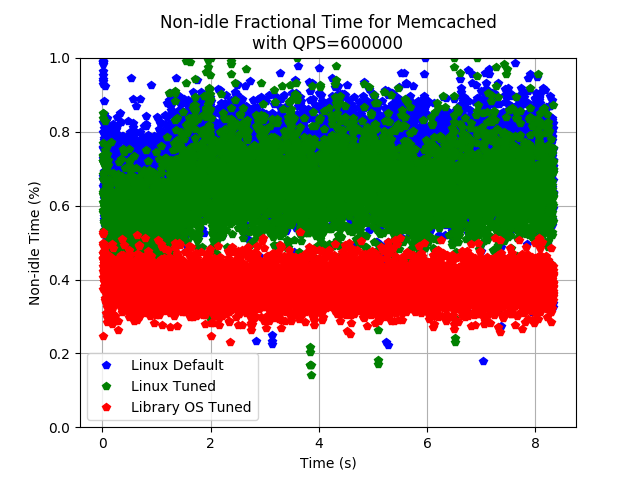
\includegraphics[width=\columnwidth]{asplos2021_figures/mcd_nonidle_QPS600000.png}
	\caption{Per interrupt measure of non-idle time computed using fixed reference cycles.}
	\label{fig:mcdnonidle600K}
\end{figure}

Experimentally, we find that, in all our applications, one can reduce the EDP by using tuned, fixed hardware parameters rather than the default Linux dynamic behaviour. Furthermore, the library OS can be tuned to achieve an even greater EDP reduction. 

In Figure~\ref{mcd600K}, we show an example EDP plot that demonstrates the time and energy trade-off of the three systems. Moreover, Figure~\ref{fig:mcdnonidle600K} typifies the details non idle time different between the library OS and Linux. Using these collected statistics, we measured total energy use at {\textasciitilde}1050 joules for {\textasciitilde}8.5 seconds (EDP = 8925 joules x second) with a 99\% tail latency of 134.4{$\mu$}s. Searching through the static settings, we find fixed hardware parameter values for Linux that save a significant {\textasciitilde}440 joules ({\textasciitilde}42\%) with a tail latency of 475{$\mu$}s.  Tuning the parameters when using the library OS yields an even greater saving of {\textasciitilde}635 joules ({\textasciitilde}60\%) with a tail latency 105{$\mu$}s. 
%These dramatic savings indicate that OS structure matters when it comes to energy efficiency, even for running IO workloads with significant idle time. Further, these results suggest that global data-center energy consumption could significantly benefit from improving operating system support for executing a single fixed and dedicated application. 

%
%
%
% ASPLOS'21 will be piloting the submission of {\it Extended
% Abstracts}. Your extended abstract — inspired by the model used for
% IEEE Micro Top
% Picks — should be {\it two pages long}, and it will be submitted separately
% from your main paper. The deadline for the extended abstract and the
% full paper will be identical. Except for the page limit, \textbf{all other
% formatting and anonymity requirements are identical} to those for full
% papers: no names or affiliations should be present, and citations should
% be anonymized if appropriate. Extended abstracts should be self-contained, though they may
% contain references to the full paper.

% We \emph{recommend}---but do not require--- that you use
% the following organization for your abstract. 
% Sections~\ref{sec:motivation} through \ref{sec:key-contributions}
% should be a summary of your full paper. Section~\ref{sec:motivation}
% motivates the paper; Section~\ref{sec:limitations} describes
% limitations of the state of the art, if applicable;
% Section~\ref{sec:key-insights} presents the key new insight or
% insights of the paper; 
% Section~\ref{sec:main-artifacts} presents the main artifacts described
% in the paper;  Section~\ref{sec:key-contributions} summarizes the key
% results and technical contributions of your paper. Finally,
% Section~\ref{sec:why-asplos} should explain why the paper is suitable
% for ASPLOS, and Section~\ref{sec:citation} should \emph{anonymously} state what its
% citation would be for a ten year test-of-time award. In
% Section~\ref{sec:revisions}, you may optionally include a paragraph
% describing how your paper has been revised, if it was previously
% submitted to another conference.

% The extended abstracts must be submitted in printable PDF format and should contain a
% {\bf maximum of 2 pages} of single-spaced two-column text, {\bf not
%   including references}.  You may include any number of pages for
% references, but we suggest you limit your bibliography to
% only the most relevant references. The extended
% abstracts should use the same formating as the regular papers. If you are using
% \LaTeX~\cite{lamport94} to typeset your extended abstract, then we suggest that
% you use \href{https://asplos-conference.org/wp-content/uploads/2020/06/asplos21-templates.zip}{this template}.
% If you use a different
% software package, then please adhere to the
% \href{https://asplos-conference.org/wp-content/uploads/2020/06/asplos21-paper-template.pdf}{formatting guidelines}
% for ASPLOS papers.

% %The \href{ https://asplos-conference.org/wp-content/uploads/2020/06/asplos21-extended-abstract-template.pdf}{sample file} for the
% %extended abstract includes guidelines the information your abstract
% %should include. 


% %The references section of your extended abstract will not count
% %towards the two page limit. We suggest you limit your bibliography to
% %only the most relevant references~\cite{lamport94}.
% The extended abstract should not have an abstract. Start with Section~\ref{sec:motivation}.

% \section{Motivation}
% \label{sec:motivation}


% \begin{itemize}
% \item What is the problem your work attacks? Be specific.
% \item Why is it an important problem?
% \end{itemize}

% \vspace{1em}

% \noindent
% Articulate the importance of this problem to the broader ASPLOS
% community, using as little jargon as possible. \emph{Be specific}
% about the problem you are addressing; it should be the one that your
% paper directly addresses.

% \section{Limitations of the State of the Art}
% \label{sec:limitations}

% \begin{itemize}
% \item What is the state of the art in this topic today (if any)?
% \item What are its limits?
% \end{itemize}

% \section{Key Insights}
% \label{sec:key-insights}

% \begin{itemize}
% \item What are the one or two key new insights in this paper?
% \item How does it advance the state of the art?
% \item What makes it more effective than past approaches?
% \end{itemize}

% \section{Main Artifacts}
% \label{sec:main-artifacts}

% \begin{itemize}
% \item What are the key artifacts presented in your paper: a
%   methodology, a hardware design, a software algorithm, an
%   optimization or control technique, etc.?
%   \item How were your artifacts implemented and evaluated? 
% \end{itemize}

% \section{Key Results and Contributions}
% \label{sec:key-contributions}

% \begin{itemize}
%   \item What are the most important \emph{one or two} empirical or theoretical
%     results of this approach?
%   \item What are the contributions that this paper makes to the state of the
%     art? List them in an \texttt{itemize} section. Each contribution should be no more than a few sentences long.
%   \item Clearly describe its advantages over past work, including how it overcomes their limitations.
% \end{itemize}


% \section{Why ASPLOS}
% \label{sec:why-asplos}

% ASPLOS emphasizes multidisciplinary research; explain how this
%   paper emphasizes synergy of \emph{two or more ASPLOS areas}: architecture,
%   programming languages, operating systems, and related areas (broadly
%   interpreted).

% \noindent
% If you are unsure whether your paper falls within the scope of ASPLOS,
% please check with the program chairs -- ASPLOS is a broad,
% multidisciplinary conference and encourages new topics.

% \section{Citation for Most Influential Paper Award}
% \label{sec:citation}

% Provide the citation for your paper if it won a Most Influential
% Paper award. You can find example citations
% on the \href{https://www.sigops.org/awards/hof/}{SIGOPS Hall of Fame}
% and \href{https://www.sigplan.org/Awards/PLDI/}{PLDI most influential
%   paper list}.  Limit the citation to 1-3 sentences
% \emph{Recall that your citation here must be anonymous}; do not include names or affiliations.

% %  \url{https://rb.gy/hd1hms}).

% \section{Revisions}
% \label{sec:revisions}

%  \emph{Optional:} Describe how this paper has been revised, if it was previously submitted to another conference.

 
% \pagebreak
\bibliographystyle{plain}
\bibliography{references}


\end{document}

